\chapter{Stratified Populations: 
Multi-session and Multi-site Data}
\markboth{Stratified Population Models}{}
\label{chapt.hscr}

\vspace{0.3cm}


In this chapter, we describe SCR models for situations when we have
multiple, distinct groups, strata or ``sessions'' (multi-session
models using the \mbox{\tt secr} terminology) indexed by a
stratum-specific population size parameter $N_{g}$. The models are
extremely general and provide a flexible hierarchical modeling
framework for modeling abundance \citep{converse_royle:2012,
  royle_etal:2012arXiv} whether with spatial or ordinary
capture-recapture models.  We believe that such ``stratified''
populations are extremely commonplace, yet most SCR applications have
been based on models that are distinctly single-population
models. This is done either by analyzing seperate data sets
one-at-a-time, producing many, if not dozens, of independent estimates
of abndance, or by pooling data from multiple study areas.  A standard
example that arises frequently is that in which multiple distinct
patches (often refuges, parks or reserves) are sampled independently
with the goal of estimating the population size in each reserve. It
makes sense to combine the data together into a single model that
permits the sharing of information about some parameters, but provides
individual estimates of abundance for each land unit.  A similar
situation is that in which a number of replicate trap arrays are
located within a landscape, sometimes for purposes of evaluating
management actions or landscape structure. This is a common situation
in studies of small mammals \citep{converse_etal:2006jwm,
  converse_etal:2006ea, converse_royle:2012}, or in mist-netting of
birds \citep{desante_etal:1995} (XXXX BETTER REF HERE WOULD BE NICE
XXXX), but there are examples of large-scale monitoring of carnivores
and other species too, e.g., tigers \citep{jhala_etal:2011}.

In the stratified population models we consider here, an individual is
assumed to be a member of a single strata, so that the population
sizes $N_{g}$ for stratum $g$ are independent of one another. However,
stratifed or multi-session SCR models are also directly relevant when
the grouping is based on distinct time samples, either periods within
a biological season, or even across years. In this case, individuals
might belong to multiple of the strata, but, the models discussed in
this chapter we not acknowledge that explicitly.
%Even with a single study
%area or trap array, it would be common to conduct multiple samples
%over short intervals, but then repeat sampling again some weeks or
%months later, and perhaps on multiple years.  
Unlike the case in which the strata represent spatial units, with
temporally defined strata, we imagine a fully dynamic, or
demographically open model for $N$ might be appropriate -- one that
involves survival and recruitment. We deal with those models
specifically in Chapt. \ref{chapt.open}.  However, the stratified
models covered here can be thought of as a primative type of model for
open systems, but in which the populations are assumed to be {\it
  independent}. Whereas the underlying model may be one of Markovian
dynamics (survival, recruitment), we could {\it ignore} that
dependence for convenience or perhaps because the dynamics are not
distinctly estimable because individual recapture rate is low, or in
order to save a few parameters. Instead of having 1 recruitment and 1
survival parameter for each year after the first, the multi-session
model only requires 1 additional parameter.

In previous chapters, we've analyzed data for a number of examples
that fall into this kind of stratified situation. In
Chapt. \ref{chapt.poisson-mn}, we analyzed the ovenbird data as an
example of a multi-catch (independent multinomial) model, where we
used year as the stratification variable, and the possum data set
(illustrating the single-catch situation). In
Chapts. \ref{chapt.covariates} and \ref{chapt.gof} we fitted models
with sex-specificity of parameters using multi-session models, where
the stratification variable in that case was sex.  In this chapter, we
focus mostly on Bayesian analysis of stratified SCR models using data
augmentation \citep{royle_etal:2012arXiv,royle_converse:2013}.  The
technical modification of data augmentation to deal with such models
is that it is based on a model for the joint distribution of the
stratum-specific population sizes, $N_{g}$, {\it conditioned} on their
total. This results in a multinomial distribution which we can analyze
in some generality using data augmentation.  As a practical matter,
specification of this multinomial distribution for the $N_{g}$
parameters {\it induces} a distribution for an individual covariate,
say $g_{i}$, which is ``group membership''.  This is extremely handy
to analyze by MCMC in the various {\bf BUGS} engines that you are
familiar with by now.  The {\bf R} package \mbox{\tt secr} fits a
class of multi-session models which we have already seen
(Sec. \ref{mle.sec.multisession}), and we used this class of models to
analyze several case studies using the multi-session models in
\mbox{\tt secr} (Sec. \ref{poisson-mn.sec.ovenbird}, XXX possum XXXX
XXXXX sex-effects XXXXX). Later in this chapter we will provide a
Bayesian analysis of the ovenbird data in {\bf BUGS} using an
analogous class of models.



\section{Stratified Data Structure}


We suppose that $g=1,2,\ldots,G$ populations, having sizes $N_{g}$,
and state-spaces ${\cal S}_{g}$, are sampled using some capture-recapture
method producing sample sizes of $n_{g}$ unique individuals and
encounters $y_{ijk}$ for individual $i=1,2,\ldots, \sum_{g=1}^{G}
n_{g}$.  Right now we won't be concerned with the details of every
type of capture-recapture observation model so, for context, we
consider the Bernoulli model in which individual and trap-specific
encounter frequencies are binomial counts: $y_{ij} \sim
\mbox{Binomial}(K,p_{ij})$.  Let $g_{i}$ be a covariate
(integer-valued, $1, \ldots, G$) indicating the population membership
of individual $i$. This covariate is {\it observed} for the sample of
captured individuals but not for individuals that are not captured.

To illustrate the prototypical data structure for stratified SCR data,
we suppose that a population comprised of 4 sub-populations is sampled
$K=5$ times. Then a plausible data set has the following structure:
\begin{verbatim}
      individual (i) : 1  2  3  4  5  6  7  8  9 10  
total encounters (y) : 1  1  3  1  1  2  2  4  1  1
      group (g)      : 1  1  1  2  3  3  3  3  4  4
\end{verbatim}
This data set indicates three individuals were captured in
subpopulation 1 (captured 1, 1, and 3 times), a single individual was
captured in population 2, four individuals were captured in population
3, and two individuals were captured in subpopulation 4.

A key idea discussed shortly is that assumption of certain models for
the collection of abundance variables $N_{g}$ {\it implies} a specific
model for the population membership variable $g_{i}$.  Then, the data
from all populations can essentially be pooled, and analyzed as data
from a single population with the appropriate model on $g_{i}$,
without having to deal with  the $N_{g}$ parameters in the model {\it directly}. In this
way, we can easily build hierarchical models for stratified
populations, using an {\it individual} level parameterization of the
model. Obviously this is important for SCR models as they all possess
at least onee random effect in the form of the activity center ${\bf
  s}$. Moreover, in the context of stratified or multi-session type
models, the ``population membership'' variable $g_{i}$ is a {\it
  categorical} type of individual covariate (Huggins 1989; Alho 1990;
Royle 2009).  Before considering SCR models specifically, in the next
section we talk a
little bit about the technical formulation of data augmentation for
stratified populations in the context of ordinary closed population
models. 


\section{Multinomial Abundance Models}


One of the key ideas to Bayesian analysis of multi-session models is
that we make use of multinomial models for allocating individuals into
strata or sessions. We do this because it allows us to analyze the
models by data augmentation \citep{converse_royle:2012,
  royle_converse:2013}, and it has a natural linkage to the Poisson
model, which is commonly used throughout ecology to model variation
in abundance. We demonstrate the formlation of multi-session models
using data augmentation here using ordinary closed population models
and apply the idea to SCR models shortly.

To motivate the technical famework, 
consider sampling $g=1,2,\ldots,G$ populations having
unknown sizes $N_{g}$, and we wish to impose model structure on the
population size variables using a Poisson distribution:
\begin{equation}
 N_{g} \sim \mbox{Poisson}(\lambda_{g})
\label{eq.poisson1}
\end{equation}
with
\begin{equation}
\log( \lambda_{g} ) = \beta_{0} + \beta_{1} x_{g}
\label{eq.poisson2}
\end{equation}
where $x_{g}$ is some measured attribute for population $g$.   We
could generalize this a bit by considering a random effecct in
Eq. \ref{eq.poisson2}, producing over-dispersed population
sizes $N_{g}$. For the special case of adding log-gamma noise, this
results in negative binomial models for $N_{g}$.

\begin{comment}
Under this
Poisson model, by conditioning on the total population size over all
$G$ populations, the $N_{g}$ variables have a multinomial distribution:
\begin{equation}
{\bf N} = (N_{1},\ldots,N_{G}) | \{ N_{T} =
\sum_{g} N_{g} \} \sim \mbox{Multinomial}( {\bm \pi} | N_{T}).
\label{eq.mn.N}
\end{equation}
with multinomial probabilities $\pi_{g} = \lambda_{g}/\sum_{g}
\lambda_{g}$. This relationship between Poisson and multinomial random
variables is a standard distribution theory result.
We apply data augmentation to this multinomial distribution, by
embedding it into a larger multinomial distribution. In particular,
define:
\begin{equation}
{\bf M}|M_{T} \sim \mbox{Multinom}(M_{T};  {\bm \pi} ) 
\label{eq.mn1}
\end{equation}
where $\pi_{s} = \lambda_{s}/\sum_{s} \lambda_{s}$ equivalent to those
of the target multinomial for ${\bf N}$.  We assume the ``real''
populations arise under a binomial sampling model:
\[
 N_{g} \sim \mbox{Binomial}(M_{g} , \psi)
\]
where $\psi \sim \mbox{Uniform}(0,1)$. This binomial sampling
preserves the marginal Poisson assumption \citep{takemura:1999}. That
is, $N_{s}$ is Poisson, unconditional on $M_{s}$ and, also,
conditional on $N_{T} = \sum_{s} N_{g}$, ${\bf N}$ has a multinomial
with probabilities ${\bm \pi}$ and index $N_{T}$.  Note also that
$N_{T} \sim \mbox{Binomial}(M_{T}, \phi)$ which is consistent with
data augmentation applied to total population size $N_{T}$. This
binomial sampling model can be represented, equivalently, by the set
of Bernoulli variables:
\[
 z_{i} \sim \mbox{Bern}(\psi)
\]
for $i=1,2,\ldots,M_{T}$.
\end{comment}

To develop a data augmentation scheme for this population size model, 
think about doing data augmentaiton on each
population {\it individually}, by assuming that 
\[
 N_{g} \sim \mbox{Binomial}(M_{g} , \psi)
\]
where $\psi \sim \mbox{Uniform}(0,1)$ as usual. 
A kep point is that  
we allow $M_{g}$ to be population specific but
$\psi$ is constant.
We could do this multi-population data augmentation by just picking each $M_{g}$ to
be some large integer (as we always do). However, we want to pick
$M_{g}$ in a way that imposes the correct structure on $N_{g}$. If
we want to enforce our Poisson model on $N_{g}$ from above, we
naturally choose
$M_{g}$ to be Poisson also, in which case the marginal distribution
of $N_{g}$ is also
Poisson, but with mean $\psi \exp(\beta_{0} + \beta_{1}x_{g})$.  Clearly $\psi$ and $\beta_{0}$
are confounded (See below for more discussion)
%, and to preserve the
%meaning of $\beta_{0}$ (as the intercept in the model for $N_{g}$ we
%should define $\beta_{0}^{*} = (1/\psi)*\beta_{0}.
In any case, for a collection of populations we want to model jointly,
we impose the structure that we desire for $N_{g}$ on the
super-population parameters $M_{g}$.
To implement this model at the individual level we need to get rid
of the $M_{g}$ parameters (the whole motivation of data augmentation in
the first place). So we condition on the total super-population size
$M_{T}= \sum_{g} M_{g}$ which is multinomial:
\begin{equation}
{\bf M}|M_{T} \sim \mbox{Multinom}(M_{T};  {\bm \pi} ) 
\label{eq.mn1}
\end{equation}
where ${\bf M}$ is the vector $(M_{1}, M_{2},\ldots,M_{G})$, and
 $\pi_{g} = \lambda_{g}/\sum_{g} \lambda_{g}$.
This is handy because we can implement this
model, e.g., in {\bf BUGS}, by introducing a variable $g_{i}$ for each $i=1,2,\ldots, M_{T}$
which is the ``group membership'' of each individual in the
super-population.   Then, conditional on $g_{i}$, a guy is either a
real guy, or a pseudo-guy, according to the binary data augmentation
variable $z_{i}$.  In other words, the following model, in {\bf BUGS} pseudo-code:
\begin{verbatim}
psi ~ dunif(0,1)
for(g in 1:G){
  pi[g] <- lambda[g]/sum(lambda[])
}
g[i] ~ dcat(pi[1:G])
z[i] ~ dbern(psi)
\end{verbatim}
produces a vector of population size parameters ${\bf N} = (N_{1},\ldots,N_{G})$
which are approximately, for large $M_{T}$, independent Poisson random variables. 


When we do data augmentation to the multinomial joint distribution,
the $\psi$ parameter takes the place of $N_{T}$, the total population
size (across all strata). And thus it is clear that $\psi$ is
confounded with $\exp(\beta_{0})$. 
%In other words, by constructing the
%model conditional on the total, $N_{T}$, we lose information about the
%intercept $\beta_{0}$, but this is recovered in the data augmentation
%parameter $\psi$.  
One of these parameters has to be fixed. We can set
$\beta_0 = 0$ or else we can fix $\psi$ (see Chapt. \ref{chapt.state-space}).  The constraint can be
specified by noting that, under the binomial data augmentation model
$\mathbb{E}(N_{T}) = \psi M_{T}$ and, under the Poisson model,
$\mathbb{E}(N_{T}) = \sum_{g} \exp(\beta_{0} + \beta_{1} x_{g})$ and
so we can set
\[
 \psi = \frac{1}{M_{T}} \sum_{g} \exp(\beta_{0} + \beta_{1} x_{g}).
\]
The linkage of $\beta_{0}$ and $\psi$ was also discussed in
Chapt. \ref{chapt.state-space} in the context of building spatial
models for density. In that case, $\beta_0$ was the intercept of the
intensity function and one could choose to estimate either $\beta_0$
or the data agmentation parameter $\psi$.

\begin{comment}
{\bf XXXXXX this is kind of important but its not obvious why! XXXXXX}
The equivalence of $\psi$ and $\beta_{0}$ can be thought of in terms
of pooling data from the different sub-populations. In a model with
{\it no} covariates, we could pool all of the data and estimate a
single parameter $\psi$ or $\beta_0$ but not both. In this sense,
pooling data from multiple spatial samples is justifiable (in terms of
sufficiency arguments) under a Poisson assumption on local abundance
(which was noted by Royle 2004b; Royle and Dorazio 2008, sec. 5.5.1).
\end{comment}

\subsection{Implementation in BUGS}

{\bf BUGS} implementation of data augmentation for structured
populations is straightforward. 
For each $M_{T}$ individual in the
super-population we introduce a latent variable $g_{i}$ to indicate
{\it which population} the individual belongs too, and we introduce a 2nd
variable $z_{i}$ to indicate whether the individual is a real
individual or not.  So, the latent super-population structure $M_{g}$
and the binomial sampling of those super-population sizes is
equivalently represented by the latent variable pair $(g_{i},z_{i})$
where $g_{i}$ is categorical with prior probabilities $\pi_{s}$ and
$z_{i} \sim \mbox{Bernoulli}(\psi)$.  In particular, the multinomial assumption
for the latent variables $M_{g}$ is formulated in terms of ``group
membership'' for each individual in the super-population of size $M_{T}$
according to:
\[
 g_{i} \sim \mbox{Categorical}\left( {\bm \pi} \right)
\]
with ${\bm \pi} = (\pi_{1}, \ldots, \pi_{G})$ and $\pi_{g} =
\lambda_{g}/(\sum_{g} \lambda_{g})$.  The binomial sampling is
described by the binary variables $z_{1},\ldots,z_{M_{T}}$ such that
\[
 z_{i} \sim \mbox{Bernoulli}(\psi)
\]
where $\psi$ is constrained as noted in the previous section.  
The {\bf BUGS} model specification for this individual-level
formulation of the model 
is shown in Panel \ref{panel.wbcode}
for an ordinary closed population model (model $M_{0}$).
This actually shows two equivalent formulations. In the left panel we
have $\psi$ and $\beta_{0}$ as free parameters.
The right panel shows the equivalent
model but recognizing the constraint between $\psi$ and $\beta_{0}$. 
 Running these models
using the \mbox{\tt multisession$\_$sim} function, you 
can verify that
they are not uniquely estimable. In particular, draws of $\beta_{0}$
using the formulation in the left-hand panel appear to be draws from
the prior distribution, uninformed by the data.

\begin{comment}
A second implementation of the model is suggested by combing the two
latent variables $g_{i}$ and $z_{i}$,
in effect, we do both the DA and the distribution among populations in
one step,
by creating a categorical variable with $G+1$
groups, where the last group corresponds to the excess zeros. 
This amounts to declaring, for the group membership variables:  
\begin{equation}
g_{i}  \sim \mbox{Categorical}( {\bm \pi}^{+} ) \mbox{ for
  $i=1,\ldots,M_{T}$}  \label{eq.parm1c}
\end{equation}
where 
the probabilities are $\pi_{s}^{+} = \pi_{s} \psi$
for $g=1,2,\ldots,G$ and $\pi_{G+1}^{+} = (1-\psi)$.
%% NOTE: This actually amounts to a very informative prior
%% distribution on N_{g} -- this is the same as for the JS model
%% described in Ch. 10 of Royle and Dorazio.
\end{comment}

\begin{panel}[htp]   
\renewcommand{\baselinestretch}{1.0}
\centering
\rule[0.15in]{\textwidth}{.03in}
\begin{tabular}{cc}
Implementation 1 & Implementation 2 \\
\begin{minipage}{2.5in}
{\small
\begin{verbatim}
model {
# This will show that psi and b0 
#   are confounded. 
  p ~ dunif(0,1)
  beta0 ~ dnorm(0,.1)
  beta1 ~ dnorm(0,.1)
  psi ~ dunif(0,1)
  for(j in 1:G){
    log(lam[j]) <- beta0 + beta1*x[j]
    gprobs[j] <- lam[j]/sum(lam[1:G])
  }
  for(i in 1:M){
    g[i] ~ dcat(gprobs[])
    z[i] ~ dbern(psi)
   mu[i] <- z[i]*p
   y[i] ~ dbin(mu[i],K)
  }
  N <- sum(z[1:M]) 
}
\end{verbatim}
}
\end{minipage}
&
\begin{minipage}{2.5in}
{\small
\begin{verbatim}
model {
# This version constrains psi with 
#   the intercept parameter
  p ~ dunif(0,1)
  beta0 ~ dnorm(0,.1)
  beta1 ~ dnorm(0,.1)
  psi <- sum(lam[])/M
  for(j in 1:G){
    log(lam[j]) <- beta0 + beta1*x[j]
    gprobs[j] <- lam[j]/sum(lam[1:G])
  }
  for(i in 1:M){  
    g[i] ~ dcat(gprobs[])
    z[i] ~ dbern(psi)
   mu[i] <- z[i]*p
   y[i] ~ dbin(mu[i],K)
  }
  N <- sum(z[1:M]) 
}
\end{verbatim}
}
\end{minipage}
\end{tabular}
\rule[-0.15in]{\textwidth}{.03in}
\caption{BUGS model specification for a capture-recapture model with
  constant encounter probability and Poisson subpopulation sizes,
  $N_{g}$, with mean depending on a single covariate \mbox{\tt x[j]}. 
Two version of the model: The first one describes the model in terms
of the intercept $\beta_0$ and DA parameter $\psi$, which are
confounded. The required constraint is indicated in the specification
on the RHS. 
}
\label{panel.wbcode}
\end{panel}

\subsection{
Simulating group structured 
capture-recapture data
}

It is helpful, as always, to simulate some data in order to understand
the model. Suppose we carry-out a camera trapping study of some
carnivore in 20 forest, using a 5 x 5 array of traps. Here we will
consider an ordinary closed population model, model $M_0$, and we
suppose there is 
some covariate, say $\mbox{Dist} = $ disturbance regime, perhaps measured by an
index of trail density or something.
We imagine a model like this:
\begin{eqnarray*}
N_{g} &\sim& Poisson(\lambda_{g})  \\
log(lambda_{g})& = &\beta_{0} + \beta_{1} \mbox{Dist}_{g} 
\end{eqnarray*}
We simulate some population sizes and encounter data  as
follows.
\begin{verbatim}
set.seed(2013)
G<- 20                          # G = 20 groups or strata
beta0<- 3
beta1<- .6
p<- .3
K<- 5                           # Sample occasions for capture-recapture
Dist<- rnorm(G)                 # Simulate covariate
lambda<- exp(beta0+beta1*Dist)  # Simulate poplation sizes 
N<-rpois(G,lambda=lambda)

y<-NULL                         # Simulate model M0 data
for(g in 1:G){
if(N[g]>0)
 y<-c(y,  rbinom(N[g],K,p))
}
g<- rep(1:G,N)

## Now keep the group id and encounter frequency only for
##   individuals that are captured 
g<-g[y>0]
y<-y[y>0]
\end{verbatim}
Thats it,
we just simulated population structure for $G=20$ populations, and
capture-recapture data for all individuals in the population. To fit
this model, we need to augment the \mbox{\tt g} and \mbox{\tt y} data
objects, and then we can run the model in {\bf JAGS} or {\bf WinBUGS}
using either specification given in Panel \ref{panel.wbcode}.
We have a script (see the help file \mbox{\tt ?multisession\_sim})
that does this.



\section{Other Approaches to Multi-Session Models}


The multinomial allows for the joint modeling of a collection of
population sizes using data augmentation.  However, as we 
demonstrated in Sec. \ref{poisson-mn.sec.ovenbird}, we can anlyze the models by putting
independent binomial priors on each $N_{g}$ and doing the data
augmentation independently for each population by itself. 
This is not any more or less difficult than the multinomial
formulation but, we imagine, it could be slightly less efficient
computationally. 
In this case we could build in amoung-group structure by modeling 
the DA parameter $\psi$ as being
variable for each subject,  as a function of group-specific variables
\citep[see][for an example]{hendriks_etal:2013}.
For example, if $C_{g}$ is the value of some stratum
covariate, then we could have $z_{i} \sim \mbox{Bernoulli}( \psi_{i})$
with
\[
 \mbox{logit}(\psi_{i}) = \beta_0 + \beta_1  C_{g_{i}}
\]
This implies a binomial model for the stratum population sizes:
\[
N_{g} \sim \mbox{Binomial}(M, \psi_{g})
\]  
(we suppose here that the population of pseudo-individuals for data
augmentation is distinct for each stratum, but constant).
%and also a multinomial for the vector 
%$N_{1}, \ldots, N_{G}, M-\sum_{g} N$ with probabilities
%$\psi_{g}$ and, for the last cell, $1-\sum_{g} \psi_{g}$. This is
%almost the same multinomial as produced by the other approach.
If $M$ is large then the $N_{g}$ are approximately
independent Poisson random variables with means $\psi_{g} M$.

As we noted in Chapt. \ref{chapt.mle}, 
the multi-session models in \mbox{\tt secr}  are based on a
Poisson prior for $N_{g}$, and then among group structure is modeled in
the parameter $\Lambda_{g}$. In our view, either model is (binomial
based on data augmentation, or Poisson) is satisfactory for any
application of capture-recapture to stratified populations.  
The main advantage of the formulation we provided here over that
implemented in \mbox{\tt secr} is we have quite a bit more flexibility
in specifying models of all sorts, either in the population size model
for $N_{g}$, or for the capture-recapture model. For example,
\citet{royle_converse:2013} fitted a model having random group effects
on encounter probability and abundance (i.e., extra-Poisson
variation). 

\section{Spatial Capture-Recapture}


The ideas described above for implementing Bayesian multi-session
models are completely general, and can be applied equally to ordinary
closed models of any sort, or spatial capture-recapture models without
any novel considerations.  \citet{royle_converse:2013} applied the
model to a small-mammal trapping problem which involved replicate
``single-catch'' arrays of traps. We review their application here,
using a simplified version of the model that can be fitted efficiently
in {\bf JAGS}.

To refresh your memory about the multinomial model, let ${\bf y}_{ik}
= (y_{i1k},y_{i2k},\ldots,y_{iJk},y_{i,J+1,k})$ be the spatial encounter history
for individual $i$, during sample occassion $k$.  
 For standard live traps (aka
``single catch'' traps), an individual can be captured in at most one
trap. Then, the vector $(y_{i1k},y_{i2k},\ldots,y_{iJk},y_{i,J+1,k})$,
where the last element $y_{i,J+1,k}$ corresponds to ``not captured'',
contains a single 1 and the remaining values are 0.  This $(J+1)\times
1$ vector ${\bf y}_{ik}$ is a multinomial trial:
\[
{\bf y}_{ik} \sim \mbox{Multinomial}(n=1; {\bm \pi}_{ik} )
\]
where ${\bm \pi}_{ik}$ is a $(J+1) \times 1$ vector where each element
represents the probability of being encountered in a trap (for
elements $1,\ldots,J$) or not captured at all (element $J+1$). Of
course, standard small-mammal traps ``fill up'' and, strictly
speaking, the multinomial distribution changes as individuals are
captured. But, as noted in Chapt. \ref{chapt.poisson-mn}, we
approximate the single catch model with the independent multinomial
model (multi-catch) to little ill-effect, as long as typical encounter
probabilities are low. The error due to misspecification of the model
can also be alleviated by using multiple traps at each point, which is
what was done in the study from which these data were obtained
\citep{converse_etal:2006ea, converse_etal:2006jwm}.

For the multinomial model, the encounter probability vector is a
function of distance between trap locations and individual activity
centers, but for this case we use the multinomial logit transform. The
equivalent half-normal model is:
\begin{equation}
\mbox{mlogit}(\pi_{ij}) = \eta_{ij}  =  \alpha_0 - \alpha_{1} \mbox{dist}({\bf x}_{j},{\bf s}_{i})^2   
\label{hscr.eq.mlogit}
\end{equation}
where $\alpha_{1} = 1/(2\sigma^2)$ and $\sigma$ is the scale
parameter of the Gaussian encounter probability model. Then, 
\[
{\bm \pi}_{ij} = \exp(\eta_{ij})/[ 1 + \sum_{j} \exp(\eta_{ij}) ]
\]
for each $j=1,2,\ldots,J$, and the last cell corresponding to the
event ``not captured'' is:
\[
\pi_{i,J+1} = 1- \sum_{j=1}^{J} \pi_{ij}
\]

There are no novel technical considerations in order to model
covariates of any time. 
For example, we usually would model a behavioral
effect in small mammal studies. For this, let
$C_{ik}$ be a covariate of previous encounter
(i.e., $C_{ik} = 0$ before the occasion of first capture, and $C_{ik}
= 1$ thereafter), then
\[
\mbox{mlogit}(\pi_{ijk}) = \eta_{ijk} = \alpha_{0}  +\alpha_{1}*\mbox{dist}({\bf  x}_{j},{\bf s}_{i})^2 +  \alpha_{2}*C_{ik}
\]
We note, in this case, the multinomial probabilities depend not only
on individual and trap, but also on sample occasion.

\subsection{Small-mammal trapping study}

We analyze data from
\citet{converse_etal:2006jwm}, from a study of the impact of
fuel reduction treatments on small mammal populations at 2 replicate
study sites in northern New Mexico (Fig. \ref{fig.studyarea}).
The data were collected 
with 
trapping over 3 years (2001-2003) in each of 4 replicate experimental
units per study site. We consider all 3 years $\times$ 4 units
$\times$ 2 sites to be model groups  (i.e., number of groups $G = 24$)
for our purposes here.

  The experimental design included plans for
thinning, burning, and thinning/burning combination treatments, as
well as a control, at each study site. However, during the period when
these data were collected, the thinning only treatment was completed
on a single experimental unit at the JM-B study area (see Converse et
al. 2006:1713), and at the JM-C study area, all 4 study experimental
units were burned in a wildfire. Both the thinning treatment and the
wildfire took place between the 2002 and 2003 study seasons.

Trapping was conducted over 10 occasions (2 per day) at each
experimental unit.
In 2001, the traps in each
experimental unit were configured in a 6 by 6 grid, with 50 m between
each trap. After a pilot project to assess the effects of trap spacing
(Converse et al. 2004) the trap density was increased such that there
was 25 m between traps, and so the grid was an 11 by 11 grid with 121
total trap stations. Multiple species were captured in the grids, but
we base our analyses on the species with the largest number of
captures, the deer mouse ({\it Peromyscus maniculatus}).
%In any case, alternate trapping locations
%included either 1 or 2 baited Sherman live traps.

The detection model is related to covariates through the multinomial
logit transform in which the trap-specific encounter probabilities are
given by Eq. \ref{eq.logit}.  In the application we have
\[
\eta_{ijk}=\alpha_{0,g_{i}} + \alpha_{1}*C_{ik}+\alpha_{2,g_{i}}*d_{ij}^{2} 
\]
where $d_{ij} \equiv dist({\bf s}_{i},{\bf x}_{j})$,
$\alpha_{0,1},\ldots, \alpha_{0,G}$ are group-specific intercepts,
$\alpha_{1}$ is the behavioral response parameter, $C_{ik}$ is a
covariate of previous encounter (i.e., $C_{ik} = 0$ before the
occasion of first capture, and $C_{ik} = 1$ thereafter), and
$\alpha_{2,g_{i}}$ is a group-specific coefficient on distance
(related to $\sigma_{g_{i}}$ by: $\alpha_{2,g_{i}} =
1/(2\sigma_{g_{i}})$), allowing for the possibility that treatments
influence home range size.

To accommodate differences in trap array configuration (e.g., $6
\times 6$ vs. $11 \times 11$ grids), we introduce a trap-operation
matrix, ${\bf A}$ where $A^{g}_{j,k}=1$ if, for group $g$, trap $j$ is
operational during period $k$ and $A^{g}_{j,k} = 0$ otherwise. A
similar approach could be used if, in practice, certain traps were not
operational during certain occasions. This could occur, for example,
if traps were sprung or damaged by animals.  Then we include trap
availability as multiplying $\exp(\eta_{ijk})$ so that, in the
multinomial logit transform, the cell probability is zeroed out for an
inoperative trap.

For the abundance model, we assume that $N_{g}$ is Poisson with mean
\[
\lambda_{g} = \exp( \beta_{0,g} +  {\bf x}'_{g} {\bm \beta} )
\]
where $\beta_{0,g}$ is a group-specific random effect (see below),
 ${\bf x}'_{g}$ is a vector of population-specific covariates,
and including an intercept.  In our analysis here, ${\bf x}_{g} = 
(\mbox{\tt year1}_{g}, \mbox{\tt year2}_{g}, \mbox{\tt thin}_{g},
\mbox{\tt fire}_{g})$ where $\mbox{\tt year1}$ and $\mbox{\tt year2}$
are dummy variables indicating years 2001 and 2002) i.e., $\mbox{\tt
  year1}_{g} = 1$ if group $g$ occurred in 2001, $\mbox{\tt
  season2}_{g} = 1$ if group $g$ occurred in 2002; \mbox{\tt thin} and
\mbox{\tt fire}
are binary treatment effects being $\mbox{\tt thin}_{g}=1$ if group $g$ was a
thinned experimental unit, and $\mbox{\tt fire}_{g} = 1$ if group $g$ was a
burned experimental unit.

We used proper uniform prior distributions for each of the regression
coefficients: $\beta_{m} \sim \mbox{Unif}(-10,10)$ for $m=1,2,3,4$,
$\alpha_{1} \sim \mbox{Unif}(-10,10)$, and $\alpha_{2} \sim
\mbox{Unif}(-10,10)$. 
For 
the group-specific intercept parameters $\beta_{0,g}$  we assumed:
\[
\beta_{0,g} \sim \mbox{Normal}(0,\tau_{\lambda})
\]
with 
$\sigma_{\lambda} = (1/\sqrt{\tau_{\lambda}}) \sim
\mbox{Unif}(0,10)$.
The mean of the normal distribution for $\beta_{0,g}$ is 0 because the
intercept of the abundance model is confounded with the data
augmentation parameter $\psi$. That is, $\psi$ is providing the
information on the total abundance which is equivalent information to
the intercept in the abundance model (Royle et al. 2012).  The effect
of this group-specific random effect is to induce extra-Poisson
variation in the group-specific abundance parameters $N_{g}$. It is
convenient to use the normal distribution on the $log(\lambda)$ scale
here but a gamma noise term multiplying $\lambda$ is equivalent to a
negative binomial abundance model (Royle et al. 2012).
 For the group-specific intercept parameter
$\alpha_{0}$ we assumed then to be independent with normal prior
\[
\alpha_{0,g}\sim \mbox{Normal}(\mu_{p},\tau_{p})
\]
and flat priors on the hyperparameters $\mu_{p}$ and
standard-deviation: $\mu_{p} \sim \mbox{Unif}(-10,10)$,
$\sigma_{p}=1/\sqrt{\tau_{p}} \sim \mbox{Unif}(0,10)$.  We assumed a
normal prior for $\alpha_{2,g}$ also, having parameters $\mu_{\alpha_{2}}$
and standard deviation $\sigma_{\alpha_{2}}$.



There was a positive response of deer mouse population density to both
thinning ($\beta_{2}$) and wildfire ($\beta_{3}$) (Table 1, Figure
1). There were also reasonably strong annual effects on
density. Overall density of the species, across all groups, was
estimated to be $0.00025$ per $m^{2}$, or 2.5 per ha. The conclusion
that both thinning and fire had a positive effect on density of
deer mice was consistent with the conclusion reached by Converse et
al. (2006).
We also found strong trap-happy responses (i.e., animals that had been
trapped previously had a higher capture probability, see $\alpha_{1}$,
in Table 1).

\begin{table}
\centering
\caption{
  Point estimates (posterior mode) and 95\% credible intervals
  for parameters in the observation
  process portion of the model as well
  as the ecological process portion of
  the model, for the joint estimation
  and modeling of density of
  Peromyscus spp. on experimental
  units at the Jemez Mountains Study
  Area, New Mexico.  See text for explanation of parameters. 
  {\bf Footnotes}: 
  (a) Only 2 fixed season effects are separately estimable.  The third
  effect =
  $ -1*(\beta_1 [seas 1]+\beta_1 [seas 2])$.
  (b) Overall abundance is summed across all 24 groups, each with an
  implied 
  area = 12.25 ha.  
  (c) Overall density is reported as individuals/m2.  
}
\begin{tabular}{lrrr}
\hline \hline
Parameter &	Estimate &	95\% Lower &	95\% Upper 
\\ \hline
Observation Process & & & \\ \hline
$\mu_{p}$        &-1.85 & -2.19 &	-1.57 \\
$\sigma_{p}$           &0.55  & 0.37  &	0.88 \\
$\alpha_1$        &0.22  & 0.05  &	0.41 \\
$\mu_{\alpha_{2}}$             &-1.28 & -1.49 &	-1.07 \\
$\sigma_{\alpha_{2}}$     &0.46  & 0.34  &		0.68 \\ \hline \hline
Ecological Process & & & \\
\hline
$\sigma_{\lambda}$      & 0.17 & 0.05  &	0.46 \\
$\beta$ [seas 1] &-0.60 & -0.80 &	-0.43 \\
$\beta$ [seas 2] &-0.17 & -0.33 &	-0.01\\
$\beta$ [seas 3](a) &0.79 & 0.59  &	0.97\\
$\beta$ [fire] &	0.60     & 0.14  &	1.03 \\
$\beta$ [thin] &	0.38     & 0.12  &	0.77 \\
N (b)&	747&	708      & 797 \\
Density (c)&2.54x10-4&2.41x10-4&	2.71x10-4 \\ \hline
\end{tabular}
\end{table}





\begin{figure}[ht]
\begin{center}
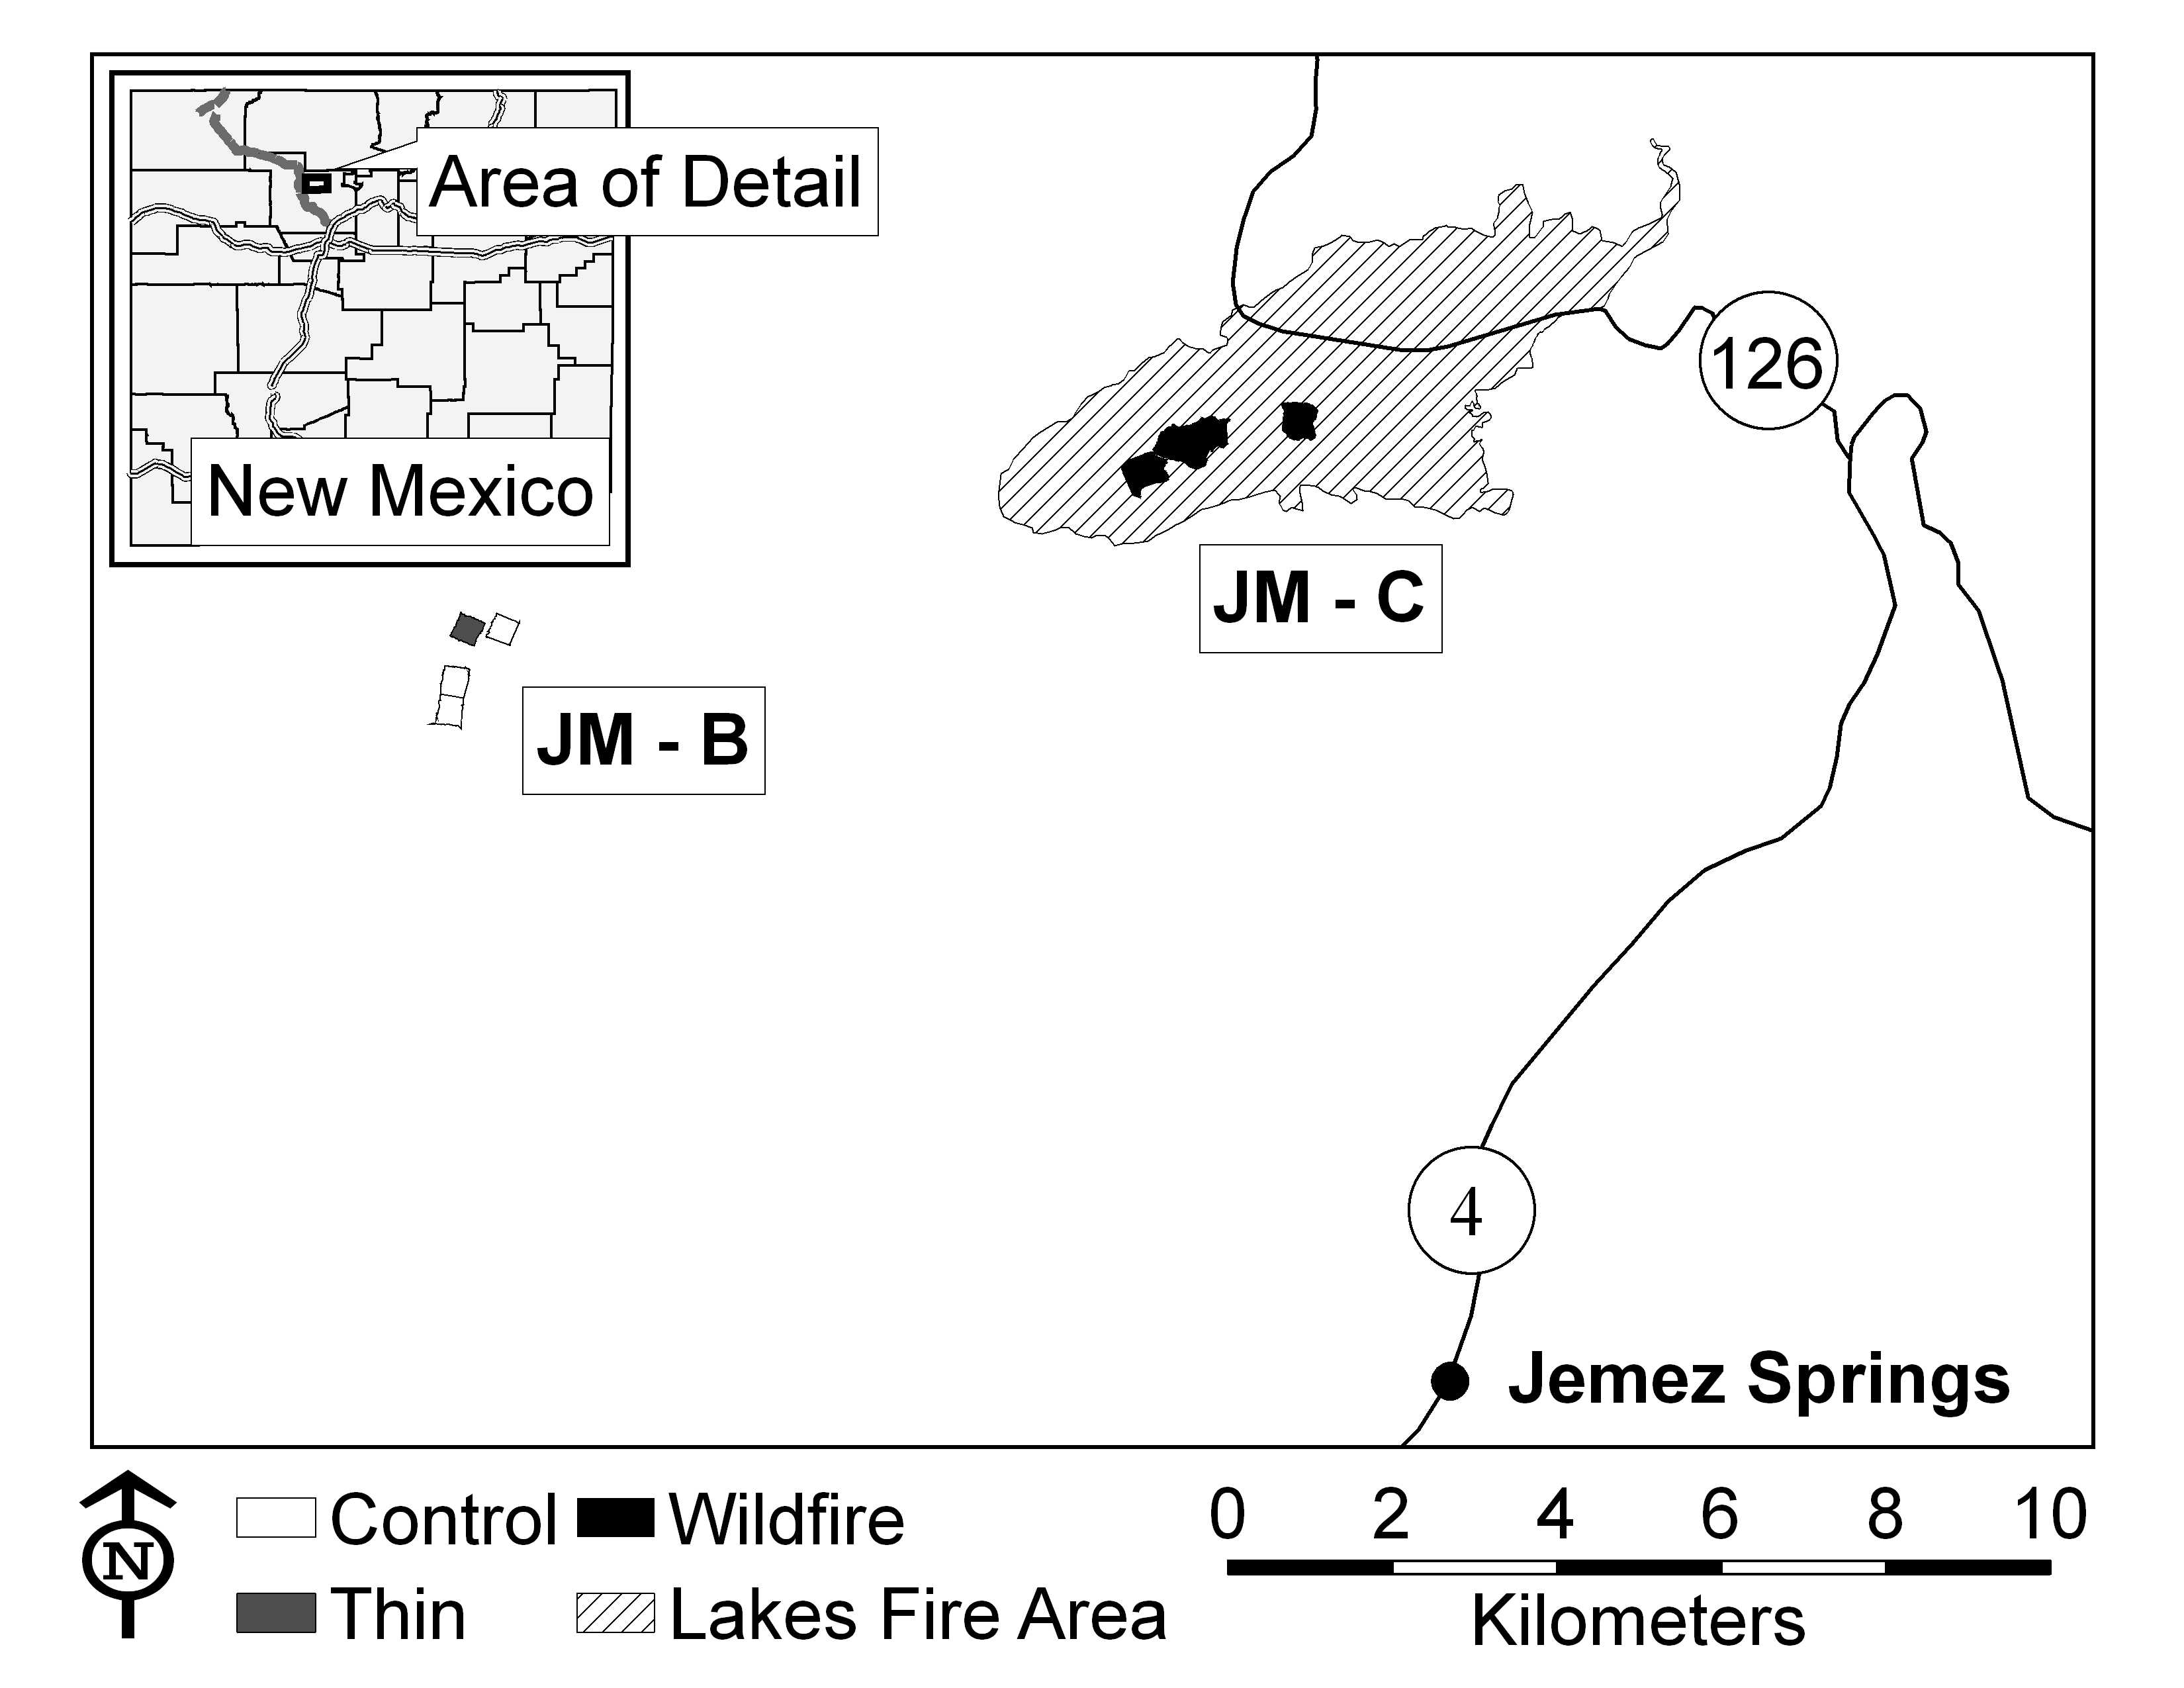
\includegraphics[height=4in,width=5.2in]{Ch14-Multisession/figs/converse_NM_Overview_4.jpg}
\end{center}
\caption{
Central New Mexico Study Area from \citet{converse_etal:2006jwm}.
}
\label{fig.studyarea}
\end{figure}



\begin{figure}[ht]
\begin{center}
\includegraphics[height=4.8in,width=6.5in]{Ch14-Multisession/figs/figure_V2.pdf}
\end{center}
\caption{
Abundance estimates for Peromyscus spp. per experimental unit
(with area = 5.0625 ha) for each of 24 groups composed of 8
experimental units in year 1 (groups 1:8), and the same 8
experimental units in year 2 (groups 9:16) and year 3 (groups 17:24)
(from \citet{royle_converse:2013}).
 Point estimates
(filled circles) are posterior modes, and error bars reflect 95\%
credible intervals. Also shown are the number of individuals
captured per group (open circles).  }
\label{fig.fig1}
\end{figure}


\subsection{Reanalysis of the Ovenbird data, but using WinBUGS}

We reanalyze the ovenbird data that we analyzed in Sec. XXXX. These
data are availabiing in secr and come from this study discussed by
Dawson XXXXXX.
The analysis before used a secr multi-session model in which $N_{t}$
was Poisson($\Lambda_{t}$) We also fitted a model in which we applied
data augmentation to {\it each} year, so that we didn't have a prior
distribution on them.  This would be simlar to the multi-session model
fitted in secr except a binomial( $\psi_{t}$M ) prior instead of
Poisson $\Lambda_{t}$.

To fit the precise Bayesian equivalent we just have to apply the DA
approach described above..................... the model is:

Results?



\section{Summary and Outlook}

Capture-recapture data are not usually collected as single isolated
studies but, instead, data are grouped or stratified in some natural
way, either because a number of distinct trap arrays are used, or
sampling occurs in several forest patches, or over time. Often this is
motivated by specific objectives, e.g., the trap arrays or units
represent experimental replicates, or sometimes just to obtain more
valid estimates of density by obtaining a representative (ideally,
random) sample of space within some region.  The fact that data are
grouped in such a way raises the obvious technical problem of having
to combine data from multiple arrays or sites in a single unified
model that accommodates explicit sources of variation in density among
sites.  This is naturally accomplished by developing an explicit model
for variation in $N$, e.g., a Poisson GLM or similar
\citep{converse_royle:2012, royle_etal:2012arXiv}. The ``design'', and
the resulting class of models, are also called multi-session models in
the package \mbox{\tt secr}, and in our analyses of
Chapt. \ref{chapt.poisson-mn} and elsewhere.

In this chapter, we outlined an approach to Bayesian analysis of
multi-session models using data augmentation, from
\citet{converse_royle:2012} and \citet{royle_converse:2013}.  This
approach allows us to build explicit models for $N$, and also gives us
great flexibility in specifying the encounter model using standard or
novel capture-recapture modeling considerations. Certain types of
multi-session models can be fitted easily in \mbox{\tt secr} and we
suspect that platform will be satisfactory for many problems you
encounter.

A common applied context of these multi-session models is when
replicate arrays are used to address explicit hypotheses about
landscape variation or modification. For example, in studies of
forestry practices, small mammal grids are used as experimental units,
and the ``dependent variable'' is $N$ (or density) for each trap
array, which is not observable.  Thus, hierarchical models are needed
to directly address the basic hypotheses of such studies.  Another
distinct context for the application of multi-session models is when
the populations are temporally structured. In these applications, we
view multi-session models as a simplified type of open population
model, an open model {\it without} explicit Markovian dynamics. They
are analogous to what are usually referred to as models of random
temporary emigration \citep{kendall_etal:1997, chandler_etal:2011}.
The models are not incorrect, just simplified, reduced versions of
more general Markovian models, and with fewer parameters to estimate.
We cover general Markovian models in Chapt. \ref{chapt.open}








\subsection{Dependence -- is it a problem?}

A standard multi-session data (e.g., the ovenbird data) is that in
which the session variable indexes time events, such as sampling in
distinct seasons or years. 
In this case, the population being sampled is the same population each
time, but subject to dynamics and movement. 

We might capture some individuals over time but we ignore the
individual recaptures across primary periods. (See Chapt. 
\ref{chapt.open}). So instead of modeling the dynamics at the individual
level we just model net change in $N_{g}$.

In time -- ignoring the dependence of $N_{g}$ probably entails a
little {\it loss} of efficiency but should have no effect on anything.
In space, there might be some individuals shared by multiple groups
and we don't think that should cause any bias or anything, even in
statement of uncertainty. So we view these models as pretty generally
useful and relevant.
A few points worht discussing: If you have grids that are in
relatively close proximity you might want to build a model in which
the total state-space is used in the model. i.e., form the union of
the state-spaces and model that. That will be more computationally
tedious but on the other hand it preserves the real landscape and any
interactions that might be affecting grids simultaneously. 

Conceptually we can apply models like this which assume Ng are
independent even if they're not... as long as we dont cear about the
underlying dynamics explictly and also possibly with some loss of
eficiency. 







